\subsection{Cut-based Analysis}

%%%%%%%%%%%%%%%%%%%%%%%%%%%%%%
\begin{figure}[!hbtp]
\centering
\subfigure[SM Higgs (cut-based) 7 TeV ]{
\centering
\label{subfig:sm_cut_7tev}
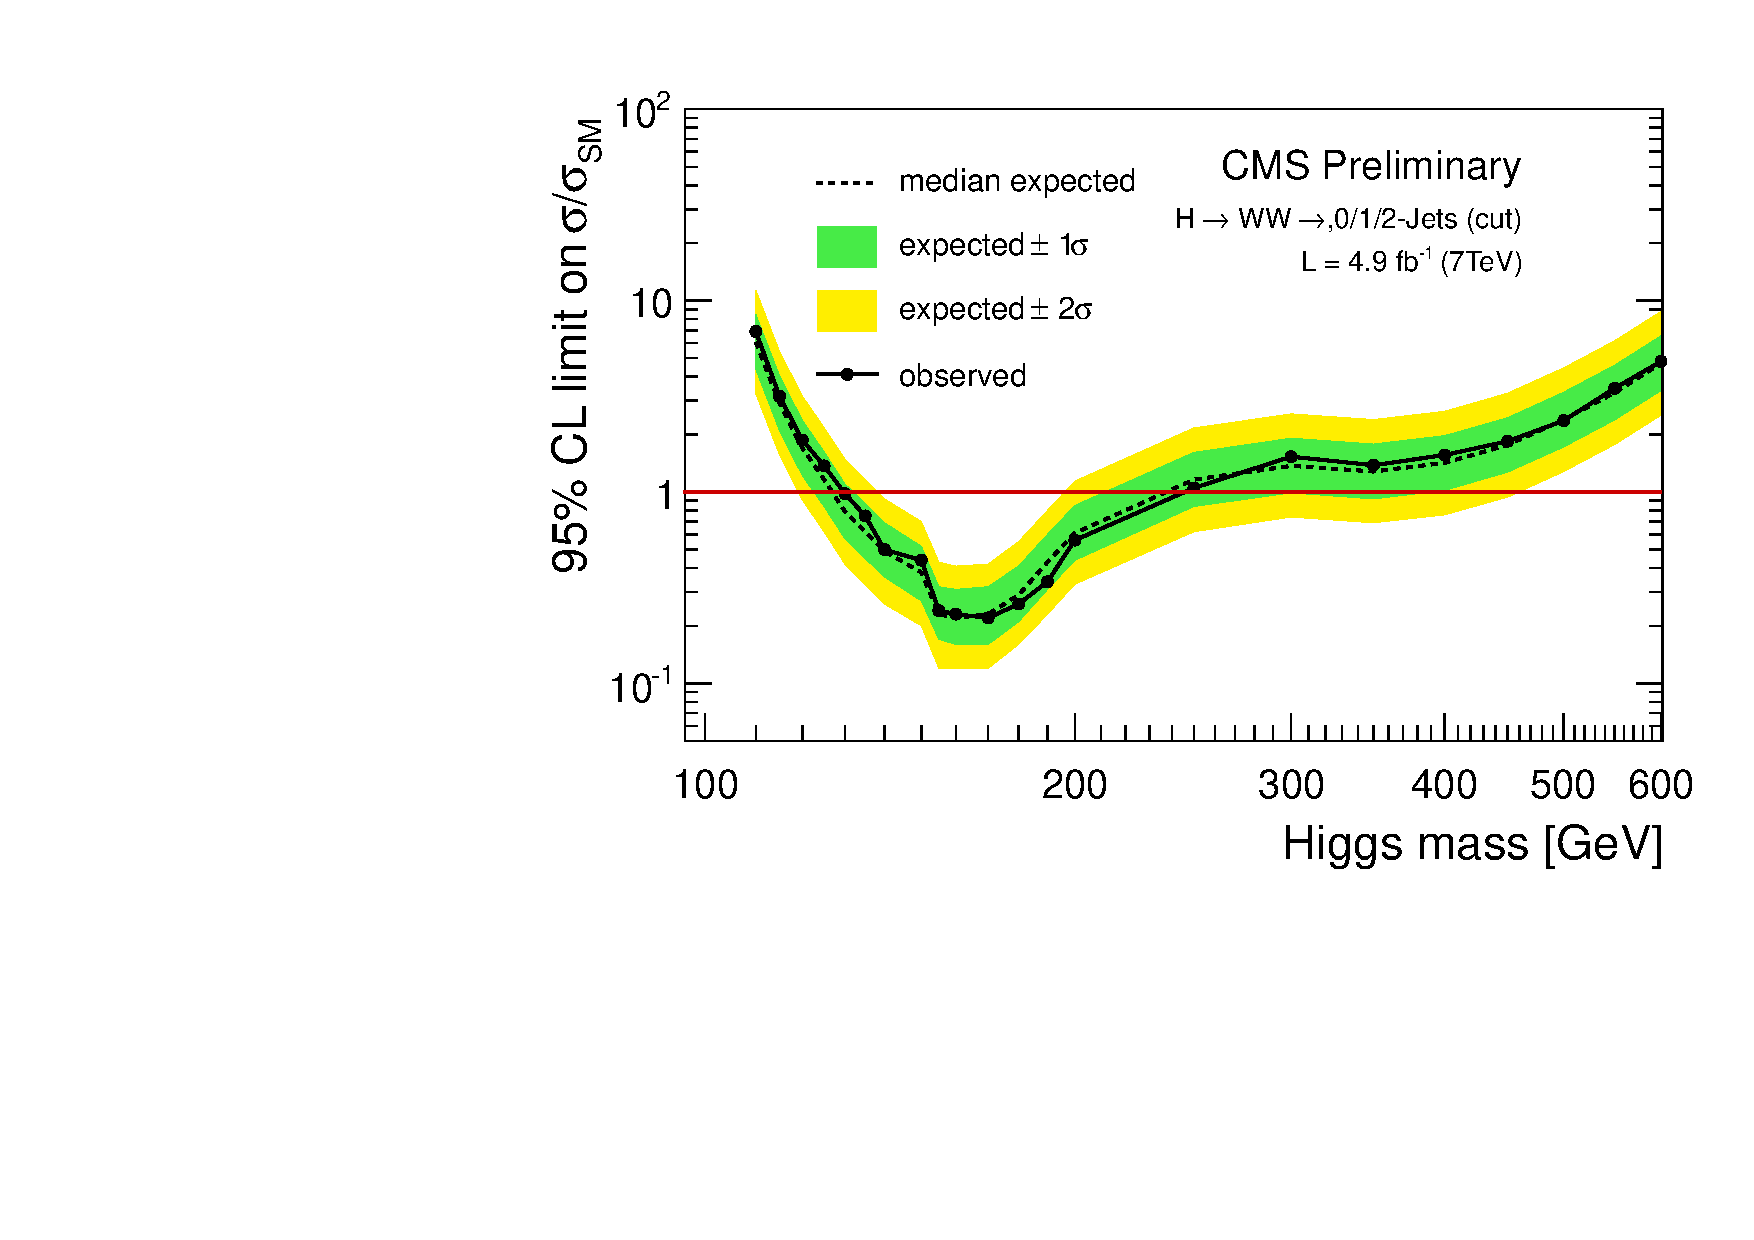
\includegraphics[width=.45\textwidth]{figures/limits_nj_cut_7TeV-CLs-asymptotic_log.pdf}}
\centering
\subfigure[SM Higgs (cut-based) 8 TeV ]{
\centering
\label{subfig:sm_cut_8tev}
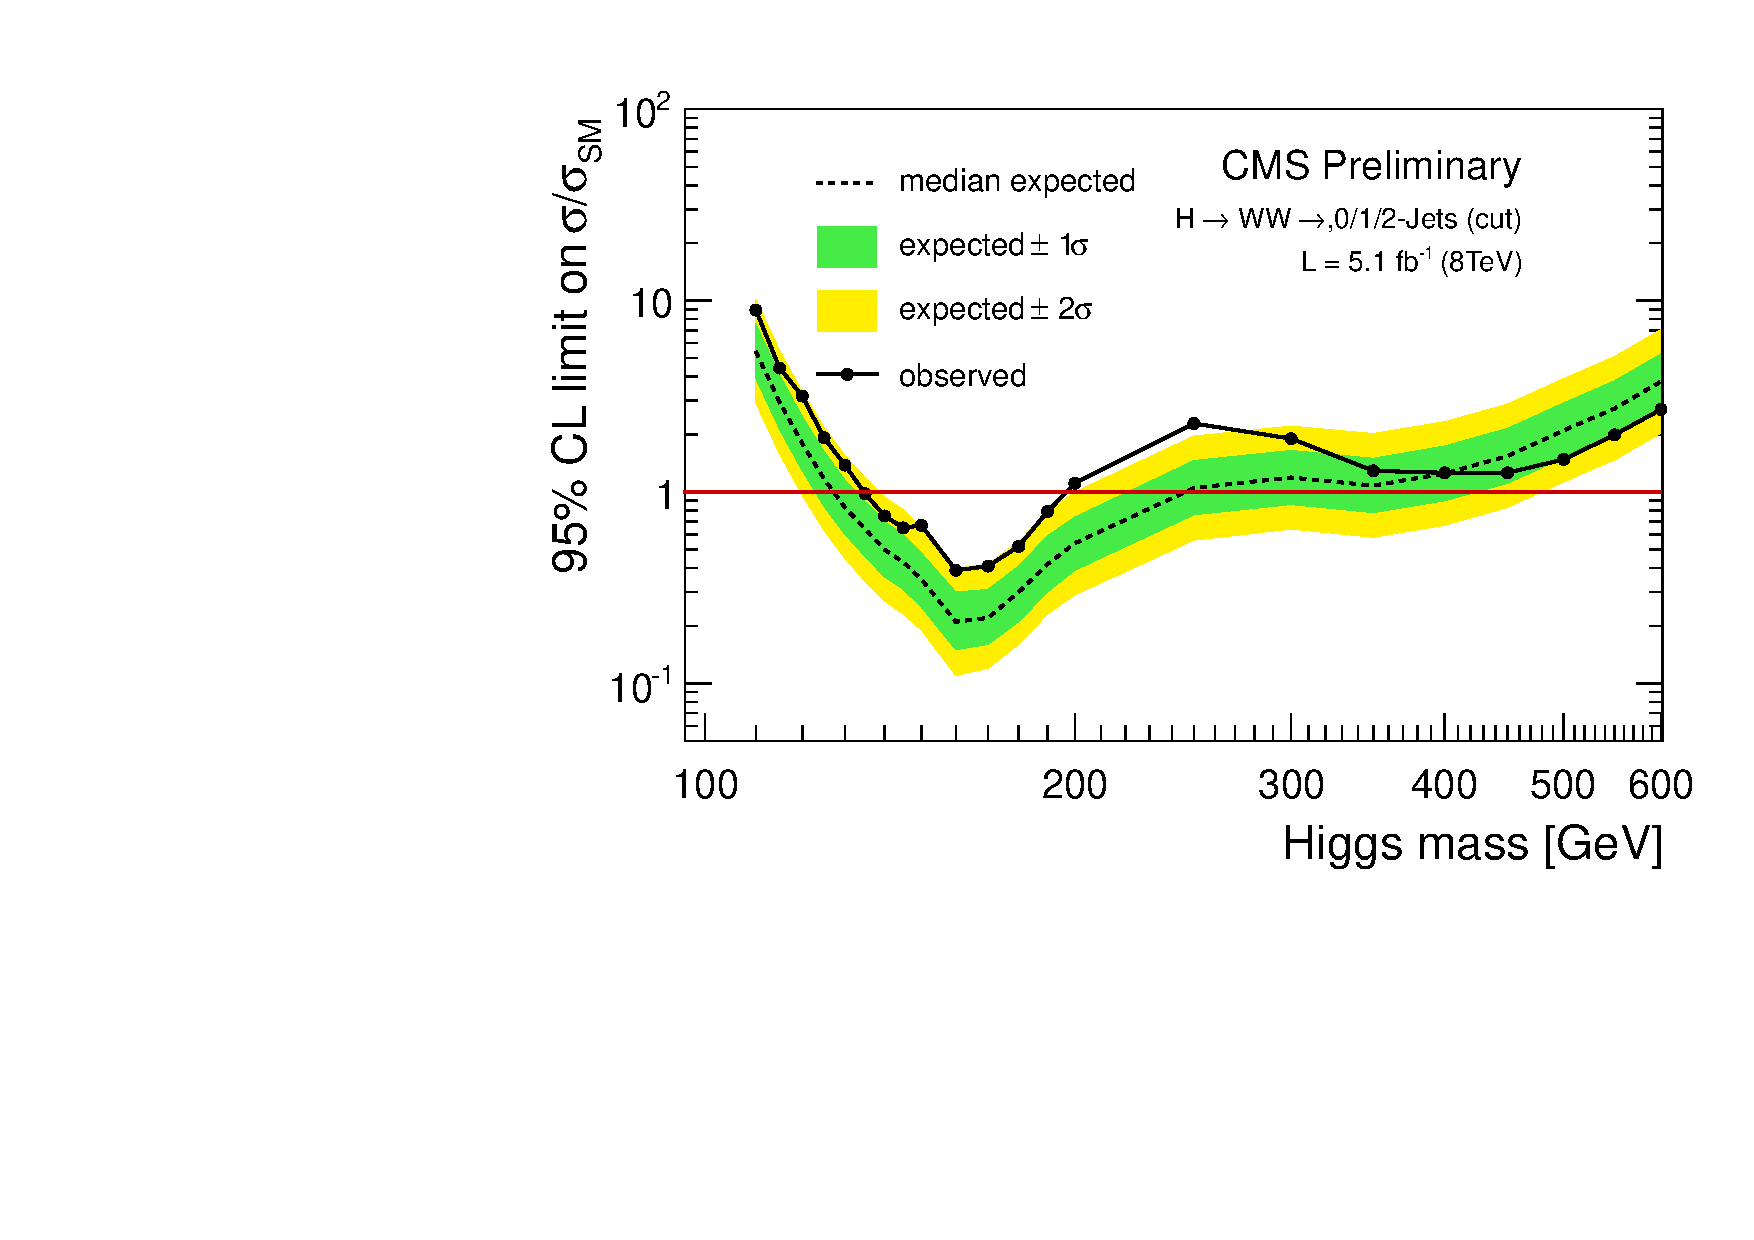
\includegraphics[width=.45\textwidth]{figures/limits_nj_cut_8TeV-CLs-asymptotic_log.pdf}} \\
\subfigure[SM Higgs (cut-based) 7+8 TeV ]{
\centering
\label{subfig:sm_cut_comb}
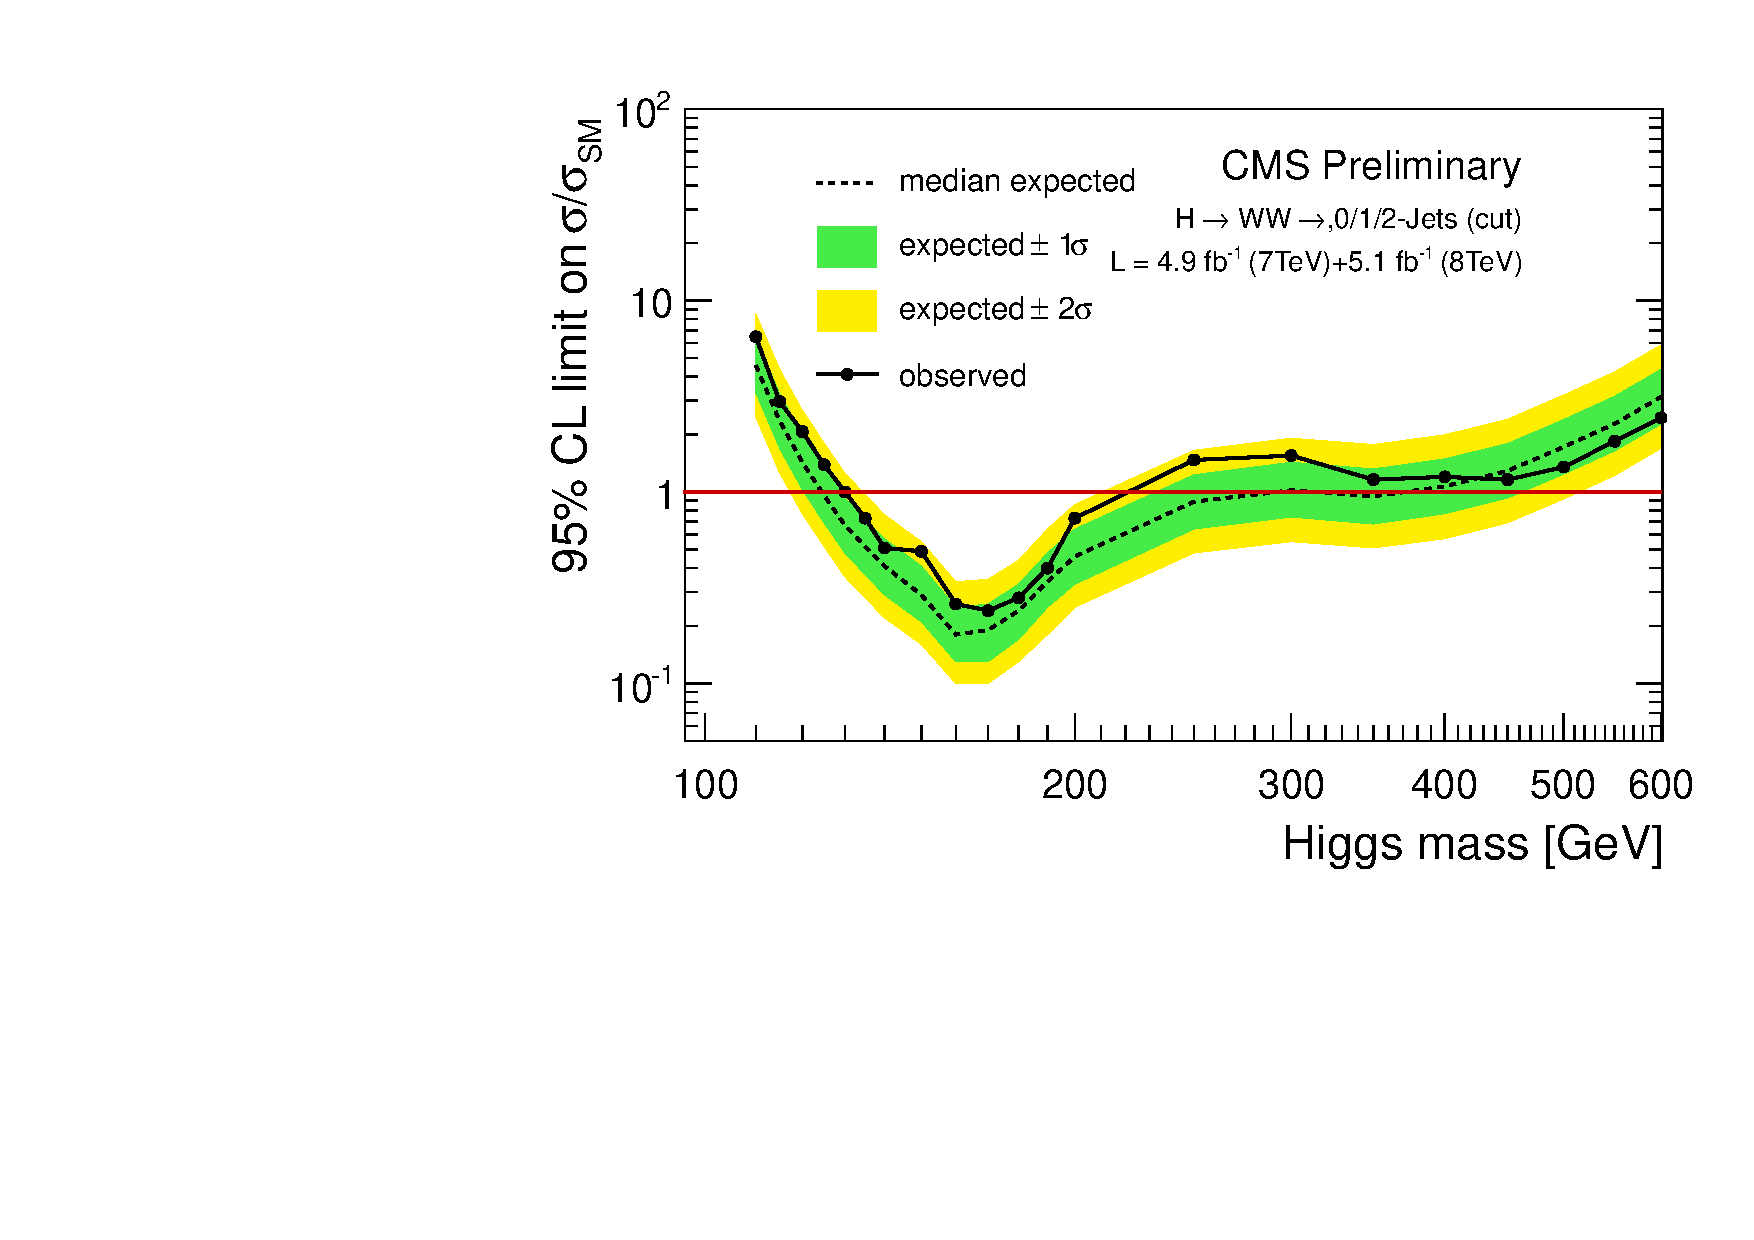
\includegraphics[width=.45\textwidth]{figures/limits_nj_cut-CLs-asymptotic_log.pdf}} \\ 
\label{fig:uls_cut}
\caption{Expected and observed upper limits for SM Higgs using the
  {\bf cut-based} analysis using 7 TeV, 8 TeV and combined data.}
\end{figure}



%%%%%%%%%%%%%%%%%%%%%%%%%%%%%%%%%%%%%%%%%%%%%%%%%%%%%%%%%%%%
\begin{table}[hbp!]
\begin{center}
\begin{tabular}{c c c c c}
\hline
\vspace{-3mm} && \\
 Higgs Mass & Observed  & Median expected & Expected range for 68\% & Expected range for 95\%   \\
\hline
\vspace{-3mm} && \\
110 & 6.89 & 6.07 & [4.37, 8.45] & [3.26, 11.33] \\
115 & 3.16 & 2.90 & [2.09, 4.04] & [1.56, 5.41] \\
120 & 1.87 & 1.70 & [1.22, 2.37] & [0.91, 3.17] \\
125 & 1.37 & 1.16 & [0.84, 1.62] & [0.62, 2.17] \\
130 & 0.98 & 0.79 & [0.57, 1.10] & [0.42, 1.48] \\
135 & 0.75 & 0.62 & [0.45, 0.87] & [0.33, 1.16] \\
140 & 0.50 & 0.49 & [0.36, 0.69] & [0.26, 0.92] \\
150 & 0.44 & 0.38 & [0.27, 0.52] & [0.20, 0.70] \\
160 & 0.23 & 0.22 & [0.16, 0.31] & [0.12, 0.41] \\
170 & 0.22 & 0.23 & [0.16, 0.32] & [0.12, 0.42] \\
180 & 0.26 & 0.29 & [0.21, 0.41] & [0.16, 0.55] \\
190 & 0.34 & 0.43 & [0.31, 0.60] & [0.23, 0.80] \\
200 & 0.56 & 0.61 & [0.44, 0.85] & [0.33, 1.14] \\
250 & 1.05 & 1.16 & [0.84, 1.61] & [0.62, 2.16] \\
300 & 1.53 & 1.37 & [0.99, 1.91] & [0.74, 2.56] \\
350 & 1.38 & 1.28 & [0.92, 1.78] & [0.69, 2.39] \\
400 & 1.56 & 1.42 & [1.02, 1.97] & [0.76, 2.64] \\
450 & 1.84 & 1.76 & [1.27, 2.44] & [0.94, 3.28] \\
500 & 2.36 & 2.39 & [1.72, 3.32] & [1.28, 4.45] \\
550 & 3.48 & 3.30 & [2.38, 4.59] & [1.77, 6.16] \\
600 & 4.81 & 4.70 & [3.39, 6.54] & [2.52, 8.77] \\
\hline
\end{tabular}
\caption{Expected and observed upper limits for SM Higgs using the
  {\bf cut-based} analysis, corresponding to $\intlumiSevenTeV$ at 7 TeV. }
\label{tab:cutbase_uls_7tev}
\end{center}
%\end{table}
%%%%%%%%%%%%%%%%%%%%%%%%%%%%%%
%\begin{table}[hbp!]
\begin{center}
\begin{tabular}{c c c c c}
\hline
\vspace{-3mm} && \\
 Higgs Mass & Observed  & Median expected & Expected range for 68\% & Expected range for 95\%   \\
\vspace{-3mm} && \\
\hline
110 & 8.92 & 5.43 & [3.91, 7.56] & [2.91, 10.13] \\
115 & 4.44 & 2.94 & [2.12, 4.09] & [1.58, 5.49] \\
120 & 3.17 & 1.79 & [1.29, 2.48] & [0.96, 3.33] \\
125 & 1.92 & 1.17 & [0.84, 1.63] & [0.63, 2.18] \\
130 & 1.38 & 0.83 & [0.60, 1.15] & [0.45, 1.55] \\
135 & 0.98 & 0.64 & [0.46, 0.89] & [0.34, 1.19] \\
140 & 0.75 & 0.50 & [0.36, 0.70] & [0.27, 0.94] \\
145 & 0.65 & 0.43 & [0.31, 0.60] & [0.23, 0.81] \\
150 & 0.67 & 0.35 & [0.25, 0.48] & [0.19, 0.65] \\
160 & 0.39 & 0.21 & [0.15, 0.30] & [0.11, 0.40] \\
170 & 0.41 & 0.22 & [0.16, 0.31] & [0.12, 0.42] \\
180 & 0.52 & 0.30 & [0.21, 0.41] & [0.16, 0.55] \\
190 & 0.79 & 0.42 & [0.30, 0.59] & [0.23, 0.79] \\
200 & 1.11 & 0.54 & [0.39, 0.74] & [0.29, 1.00] \\
250 & 2.28 & 1.05 & [0.76, 1.46] & [0.56, 1.96] \\
300 & 1.90 & 1.19 & [0.86, 1.65] & [0.64, 2.21] \\
350 & 1.29 & 1.08 & [0.78, 1.50] & [0.58, 2.02] \\
400 & 1.26 & 1.25 & [0.90, 1.74] & [0.67, 2.33] \\
450 & 1.26 & 1.54 & [1.11, 2.15] & [0.83, 2.88] \\
500 & 1.48 & 2.10 & [1.51, 2.92] & [1.13, 3.91] \\
550 & 1.99 & 2.73 & [1.97, 3.81] & [1.47, 5.10] \\
600 & 2.70 & 3.78 & [2.73, 5.26] & [2.03, 7.06] \\
\hline
\end{tabular}
\caption{Expected and observed upper limits for SM Higgs using the
  {\bf cut-based} analysis with \intlumiEightTeV\ of data at 8 TeV.}
\label{tab:cutbase_uls_8tev}
\end{center}
\end{table}
%%%%%%%%%%%%%%%%%%%%%%%%%%%%%%
\begin{table}[hbp!]
\begin{center}
\begin{tabular}{c c c c c}
\hline
\vspace{-3mm} && \\
 Higgs Mass & Observed  & Median expected & Expected range for 68\% & Expected range for 95\%   \\
\hline
\vspace{-3mm} && \\
110 & 6.47 & 4.58 & [3.30, 6.37] & [2.46, 8.54] \\
115 & 2.97 & 2.35 & [1.69, 3.27] & [1.26, 4.38] \\
120 & 2.07 & 1.43 & [1.03, 1.99] & [0.77, 2.67] \\
125 & 1.39 & 0.96 & [0.69, 1.34] & [0.52, 1.80] \\
130 & 1.00 & 0.67 & [0.48, 0.93] & [0.36, 1.25] \\
135 & 0.73 & 0.52 & [0.37, 0.72] & [0.28, 0.97] \\
140 & 0.51 & 0.41 & [0.29, 0.57] & [0.22, 0.76] \\
150 & 0.49 & 0.29 & [0.21, 0.41] & [0.16, 0.55] \\
160 & 0.26 & 0.18 & [0.13, 0.25] & [0.10, 0.34] \\
170 & 0.24 & 0.19 & [0.13, 0.26] & [0.10, 0.35] \\
180 & 0.28 & 0.24 & [0.17, 0.33] & [0.13, 0.44] \\
190 & 0.40 & 0.34 & [0.25, 0.48] & [0.18, 0.64] \\
200 & 0.73 & 0.46 & [0.33, 0.64] & [0.25, 0.86] \\
250 & 1.47 & 0.89 & [0.64, 1.23] & [0.48, 1.65] \\
300 & 1.55 & 1.02 & [0.74, 1.43] & [0.55, 1.91] \\
350 & 1.16 & 0.95 & [0.68, 1.32] & [0.51, 1.77] \\
400 & 1.20 & 1.07 & [0.77, 1.49] & [0.57, 1.99] \\
450 & 1.16 & 1.29 & [0.93, 1.79] & [0.69, 2.40] \\
500 & 1.35 & 1.72 & [1.24, 2.39] & [0.92, 3.21] \\
550 & 1.84 & 2.27 & [1.64, 3.16] & [1.22, 4.24] \\
600 & 2.44 & 3.14 & [2.26, 4.37] & [1.69, 5.86] \\
\hline
\end{tabular}
\caption{Expected and observed upper limits for SM Higgs using the
  {\bf cut-based} analysis, corresponding to $\intlumiSevenTeV$ at 7 TeV and $\intlumiEightTeV$ 8 TeV data.}
\label{tab:cutbase_uls_7and8tev}
\end{center}
\end{table}
%%%%%%%%%%%%%%%%%%%%%%%%%%%%%
\clearpage



\subsection{Shape Based Analysis}

%%%%%%%%%%%%%%%%%%%%%%%%%%%%%%
\begin{figure}[!hbtp]
\centering
\subfigure[SM Higgs (BDT shape-based) 7 TeV ]{
\centering
\label{subfig:sm_shape_7tev}
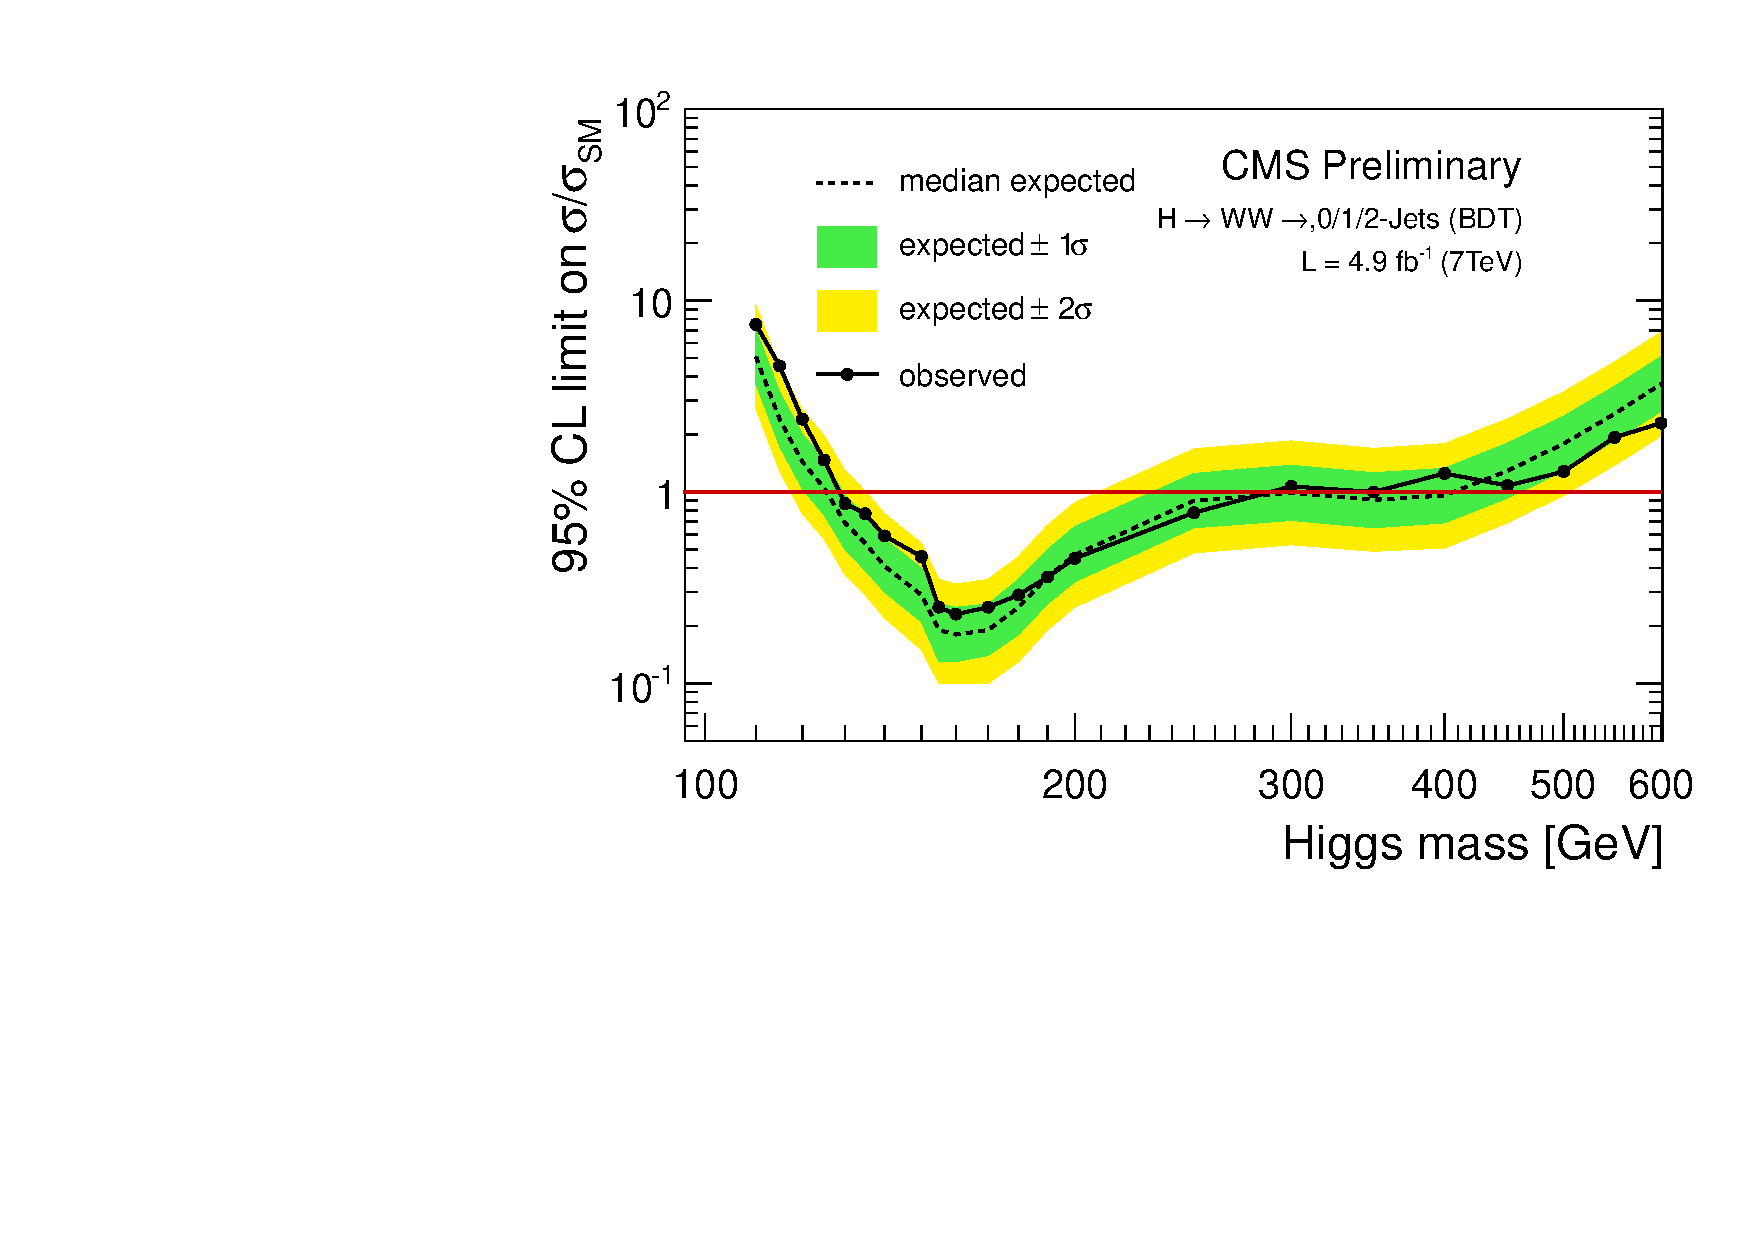
\includegraphics[width=.45\textwidth]{figures/limits_nj_shape_7TeV-CLs-asymptotic_log.pdf}}
\centering
\subfigure[SM Higgs (shape-based) 8 TeV ]{
\centering
\label{subfig:sm_shape_8tev}
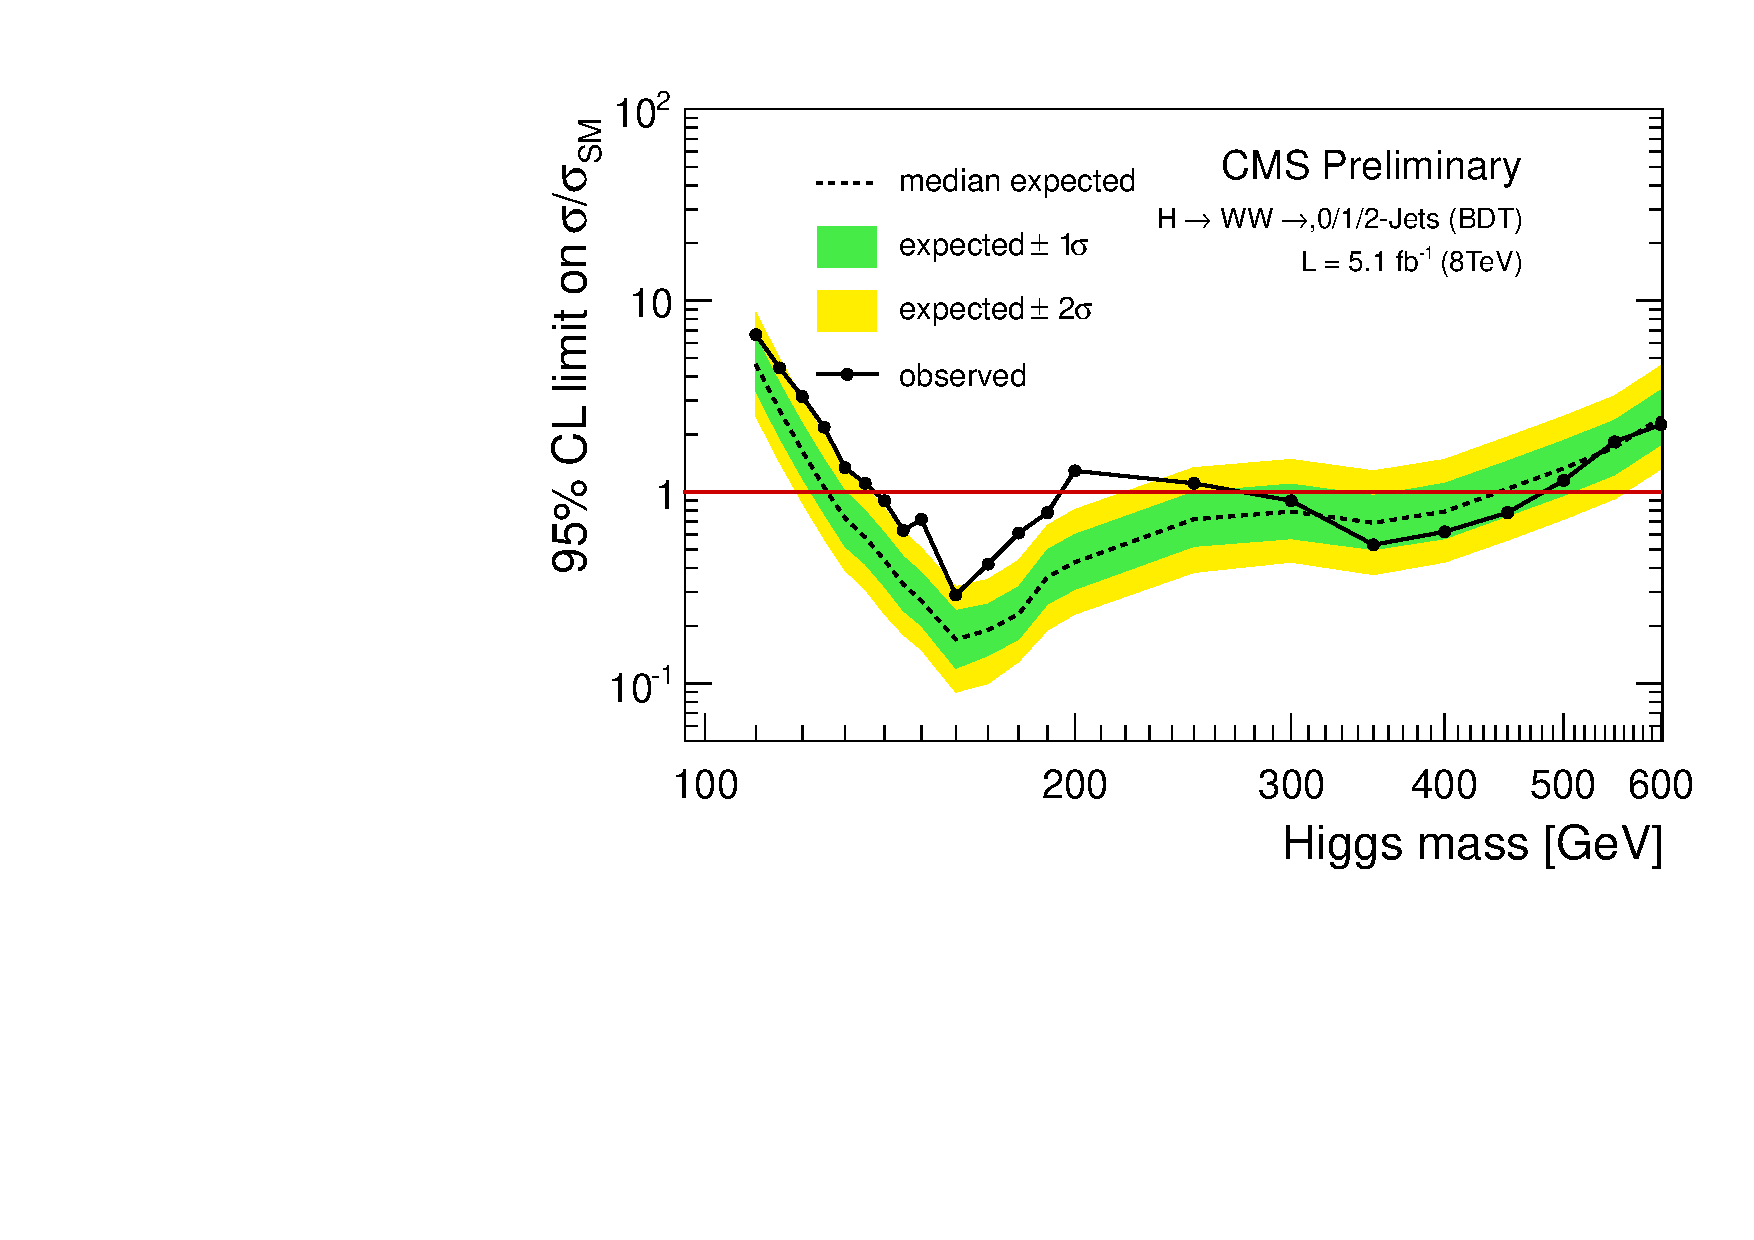
\includegraphics[width=.45\textwidth]{figures/limits_nj_shape_8TeV-CLs-asymptotic_log.pdf}} \\
\subfigure[SM Higgs (shape-based) 7+8 TeV ]{
\centering
\label{subfig:sm_shape_comb}
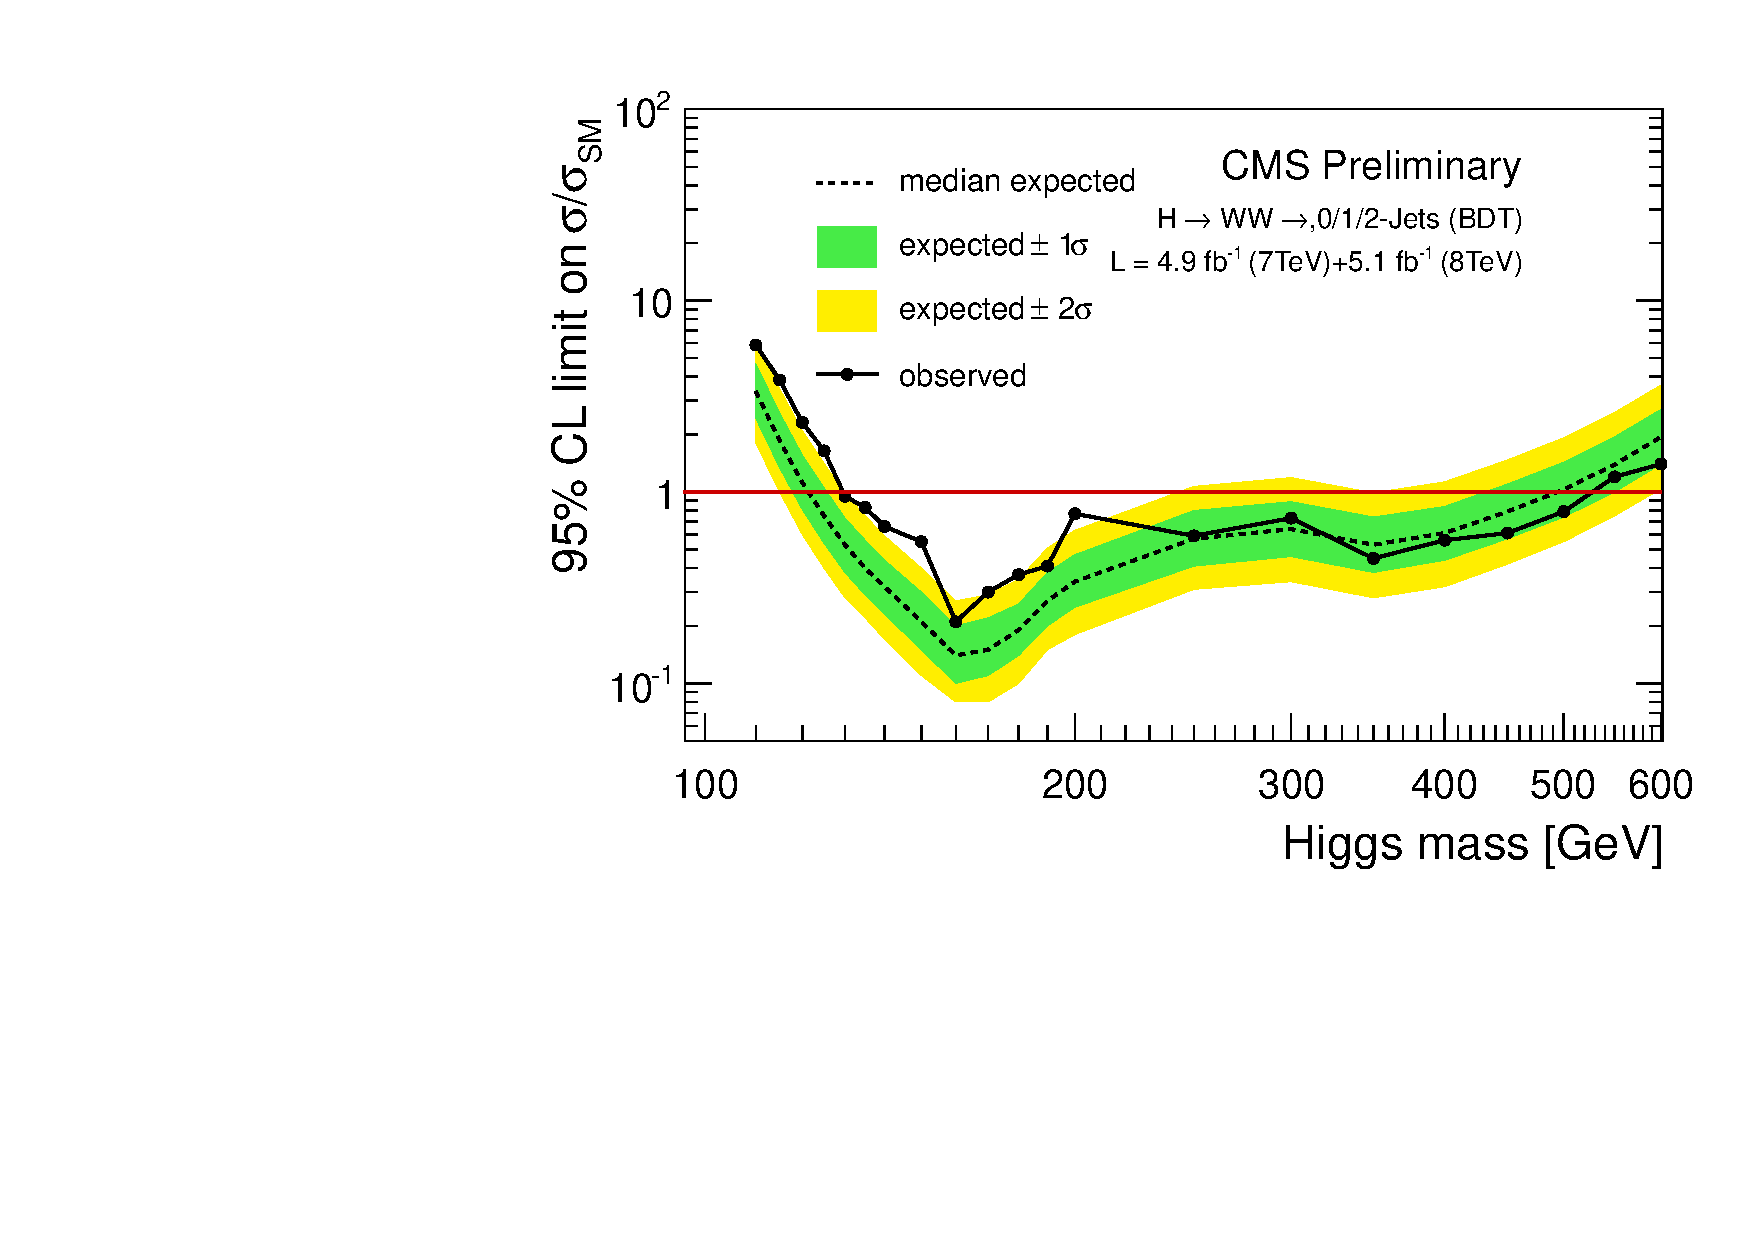
\includegraphics[width=.45\textwidth]{figures/limits_nj_shape-CLs-asymptotic_log.pdf}} \\ 
\label{fig:uls_shape}
\caption{Expected and observed upper limits for SM Higgs using the
  {\bf shape-based} analysis using 7 TeV, 8 TeV and combined data.}
\end{figure}

%%%%%%%%%%%%%%%%%%%%%%%%%%%%%%%%%%%%%%%%%%%%%%%%%%%%%%%%%%%%
\begin{table}[hbp!]
\begin{center}
\begin{tabular}{c c c c c}
\hline
\vspace{-3mm} && \\
 Higgs Mass & Observed  & Median expected & Expected range for 68\% & Expected range for 95\%   \\
\hline
\vspace{-3mm} && \\
110 & 7.51 & 5.09 & [3.67, 7.08] & [2.73, 9.49] \\
115 & 4.56 & 2.40 & [1.73, 3.33] & [1.29, 4.47] \\
120 & 2.40 & 1.44 & [1.04, 2.01] & [0.77, 2.69] \\
125 & 1.47 & 1.05 & [0.76, 1.47] & [0.57, 1.97] \\
130 & 0.87 & 0.69 & [0.50, 0.96] & [0.37, 1.29] \\
135 & 0.77 & 0.54 & [0.39, 0.76] & [0.29, 1.01] \\
140 & 0.59 & 0.41 & [0.30, 0.57] & [0.22, 0.77] \\
150 & 0.14 & 0.29 & [0.21, 0.40] & [0.15, 0.54] \\
160 & 0.23 & 0.18 & [0.13, 0.25] & [0.10, 0.33] \\
170 & 0.25 & 0.19 & [0.14, 0.26] & [0.10, 0.35] \\
180 & 0.29 & 0.25 & [0.18, 0.35] & [0.13, 0.46] \\
190 & 0.36 & 0.36 & [0.26, 0.50] & [0.19, 0.67] \\
200 & 0.45 & 0.47 & [0.34, 0.66] & [0.25, 0.88] \\
250 & 0.78 & 0.90 & [0.65, 1.25] & [0.48, 1.68] \\
300 & 1.07 & 0.99 & [0.71, 1.38] & [0.53, 1.85] \\
350 & 1.00 & 0.91 & [0.65, 1.26] & [0.49, 1.69] \\
400 & 1.25 & 0.96 & [0.69, 1.33] & [0.51, 1.79] \\
450 & 1.08 & 1.29 & [0.93, 1.80] & [0.69, 2.41] \\
500 & 1.28 & 1.79 & [1.29, 2.49] & [0.96, 3.34] \\
550 & 1.93 & 2.56 & [1.85, 3.57] & [1.38, 4.78] \\
600 & 2.29 & 3.66 & [2.64, 5.09] & [1.96, 6.83] \\
\hline
\end{tabular}
\caption{Expected and observed upper limits for SM Higgs using the
  {\bf shape-based} analysis, corresponding to $\intlumiSevenTeV$ at 7 TeV. }
\label{tab:shapebase_uls_7tev}
\end{center}
%\end{table}
%%%%%%%%%%%%%%%%%%%%%%%%%%%%%%
%\begin{table}[hbp!]
\begin{center}
\begin{tabular}{c c c c c}
\hline
\vspace{-3mm} && \\
 Higgs Mass & Observed  & Median expected & Expected range for 68\% & Expected range for 95\%   \\
\vspace{-3mm} && \\
\hline
110 & 6.64 & 4.64 & [3.34, 6.45] & [2.49, 8.65] \\
115 & 4.45 & 2.67 & [1.92, 3.71] & [1.43, 4.98] \\
120 & 3.15 & 1.64 & [1.18, 2.28] & [0.88, 3.06] \\
125 & 2.18 & 1.06 & [0.77, 1.48] & [0.57, 1.99] \\
130 & 1.34 & 0.73 & [0.52, 1.01] & [0.39, 1.35] \\
135 & 1.11 & 0.58 & [0.42, 0.80] & [0.31, 1.08] \\
140 & 0.90 & 0.44 & [0.32, 0.61] & [0.23, 0.82] \\
145 & 0.63 & 0.33 & [0.24, 0.46] & [0.18, 0.62] \\
150 & 0.72 & 0.27 & [0.20, 0.38] & [0.15, 0.51] \\
160 & 0.29 & 0.17 & [0.12, 0.24] & [0.09, 0.32] \\
170 & 0.42 & 0.19 & [0.14, 0.26] & [0.10, 0.35] \\
180 & 0.61 & 0.23 & [0.17, 0.32] & [0.13, 0.44] \\
190 & 0.78 & 0.36 & [0.26, 0.50] & [0.19, 0.67] \\
200 & 1.29 & 0.43 & [0.31, 0.60] & [0.23, 0.81] \\
% 200 & 0.34 & 0.43 & [0.31, 0.60] & [0.23, 0.81] \\ rMax = 50 for observed
250 & 1.11 & 0.72 & [0.52, 1.00] & [0.38, 1.34] \\
300 & 0.90 & 0.79 & [0.57, 1.10] & [0.43, 1.48] \\
350 & 0.53 & 0.69 & [0.50, 0.96] & [0.37, 1.29] \\
400 & 0.62 & 0.79 & [0.57, 1.11] & [0.43, 1.48] \\
450 & 0.78 & 1.04 & [0.75, 1.45] & [0.56, 1.94] \\
500 & 1.15 & 1.33 & [0.96, 1.86] & [0.72, 2.49] \\
550 & 1.83 & 1.71 & [1.23, 2.37] & [0.92, 3.18] \\
600 & 2.25 & 2.45 & [1.77, 3.41] & [1.32, 4.57] \\
\hline
\end{tabular}
\caption{Expected and observed upper limits for SM Higgs using the
  {\bf shape-based} analysis with \intlumiEightTeV\ of data at 8 TeV.}
\label{tab:shapebase_uls_8tev}
\end{center}
\end{table}
%%%%%%%%%%%%%%%%%%%%%%%%%%%%%%
\begin{table}[hbp!]
\begin{center}
\begin{tabular}{c c c c c}
\hline
\vspace{-3mm} && \\
 Higgs Mass & Observed  & Median expected & Expected range for 68\% & Expected range for 95\%   \\
\hline
110 & 5.86 & 3.35 & [2.42, 4.67] & [1.80, 6.25] \\
115 & 3.85 & 1.86 & [1.34, 2.59] & [1.00, 3.47] \\
120 & 2.31 & 1.12 & [0.81, 1.56] & [0.60, 2.09] \\
125 & 1.64 & 0.75 & [0.54, 1.05] & [0.40, 1.41] \\
130 & 0.95 & 0.53 & [0.38, 0.73] & [0.28, 0.98] \\
135 & 0.83 & 0.40 & [0.29, 0.56] & [0.22, 0.75] \\
140 & 0.66 & 0.32 & [0.23, 0.44] & [0.17, 0.59] \\
150 & 0.55 & 0.21 & [0.15, 0.30] & [0.11, 0.40] \\
160 & 0.21 & 0.14 & [0.10, 0.20] & [0.08, 0.27] \\
170 & 0.30 & 0.15 & [0.11, 0.22] & [0.08, 0.29] \\
180 & 0.37 & 0.19 & [0.14, 0.26] & [0.10, 0.35] \\
190 & 0.41 & 0.27 & [0.20, 0.38] & [0.15, 0.51] \\
200 & 0.77 & 0.34 & [0.25, 0.47] & [0.18, 0.63] \\
250 & 0.59 & 0.57 & [0.41, 0.80] & [0.31, 1.07] \\
300 & 0.73 & 0.64 & [0.46, 0.89] & [0.34, 1.19] \\
350 & 0.45 & 0.53 & [0.38, 0.74] & [0.28, 0.99] \\
400 & 0.56 & 0.61 & [0.44, 0.84] & [0.32, 1.13] \\
450 & 0.61 & 0.79 & [0.57, 1.10] & [0.42, 1.47] \\
500 & 0.79 & 1.03 & [0.74, 1.43] & [0.55, 1.92] \\
550 & 1.20 & 1.39 & [1.00, 1.94] & [0.75, 2.60] \\
600 & 1.40 & 1.94 & [1.40, 2.70] & [1.04, 3.62] \\
\hline
\end{tabular}
\caption{Expected and observed upper limits for SM Higgs using the
  {\bf shape-based} analysis, corresponding to $\intlumiSevenTeV$ at 7 TeV and $\intlumiEightTeV$ 8 TeV data.}
\label{tab:shapebase_uls_7and8tev}
\end{center}
\end{table}
%%%%%%%%%%%%%%%%%%%%%%%%%%%%%
\clearpage

